\documentclass{article}

\usepackage{graphicx}
\usepackage{tikz}
\usepackage{tikzsymbols}
\usetikzlibrary{calc,patterns,shapes.geometric}
\pagestyle{empty}
\usepackage[margin=0pt]{geometry}
\geometry{papersize={14in,12in}}

\def\centerarc[#1](#2)(#3:#4:#5){\draw[#1] ($(#2)+({#5*cos(#3)},{#5*sin(#3)})$) arc (#3:#4:#5);}

\begin{document}
	\begin{figure}
		\centering
		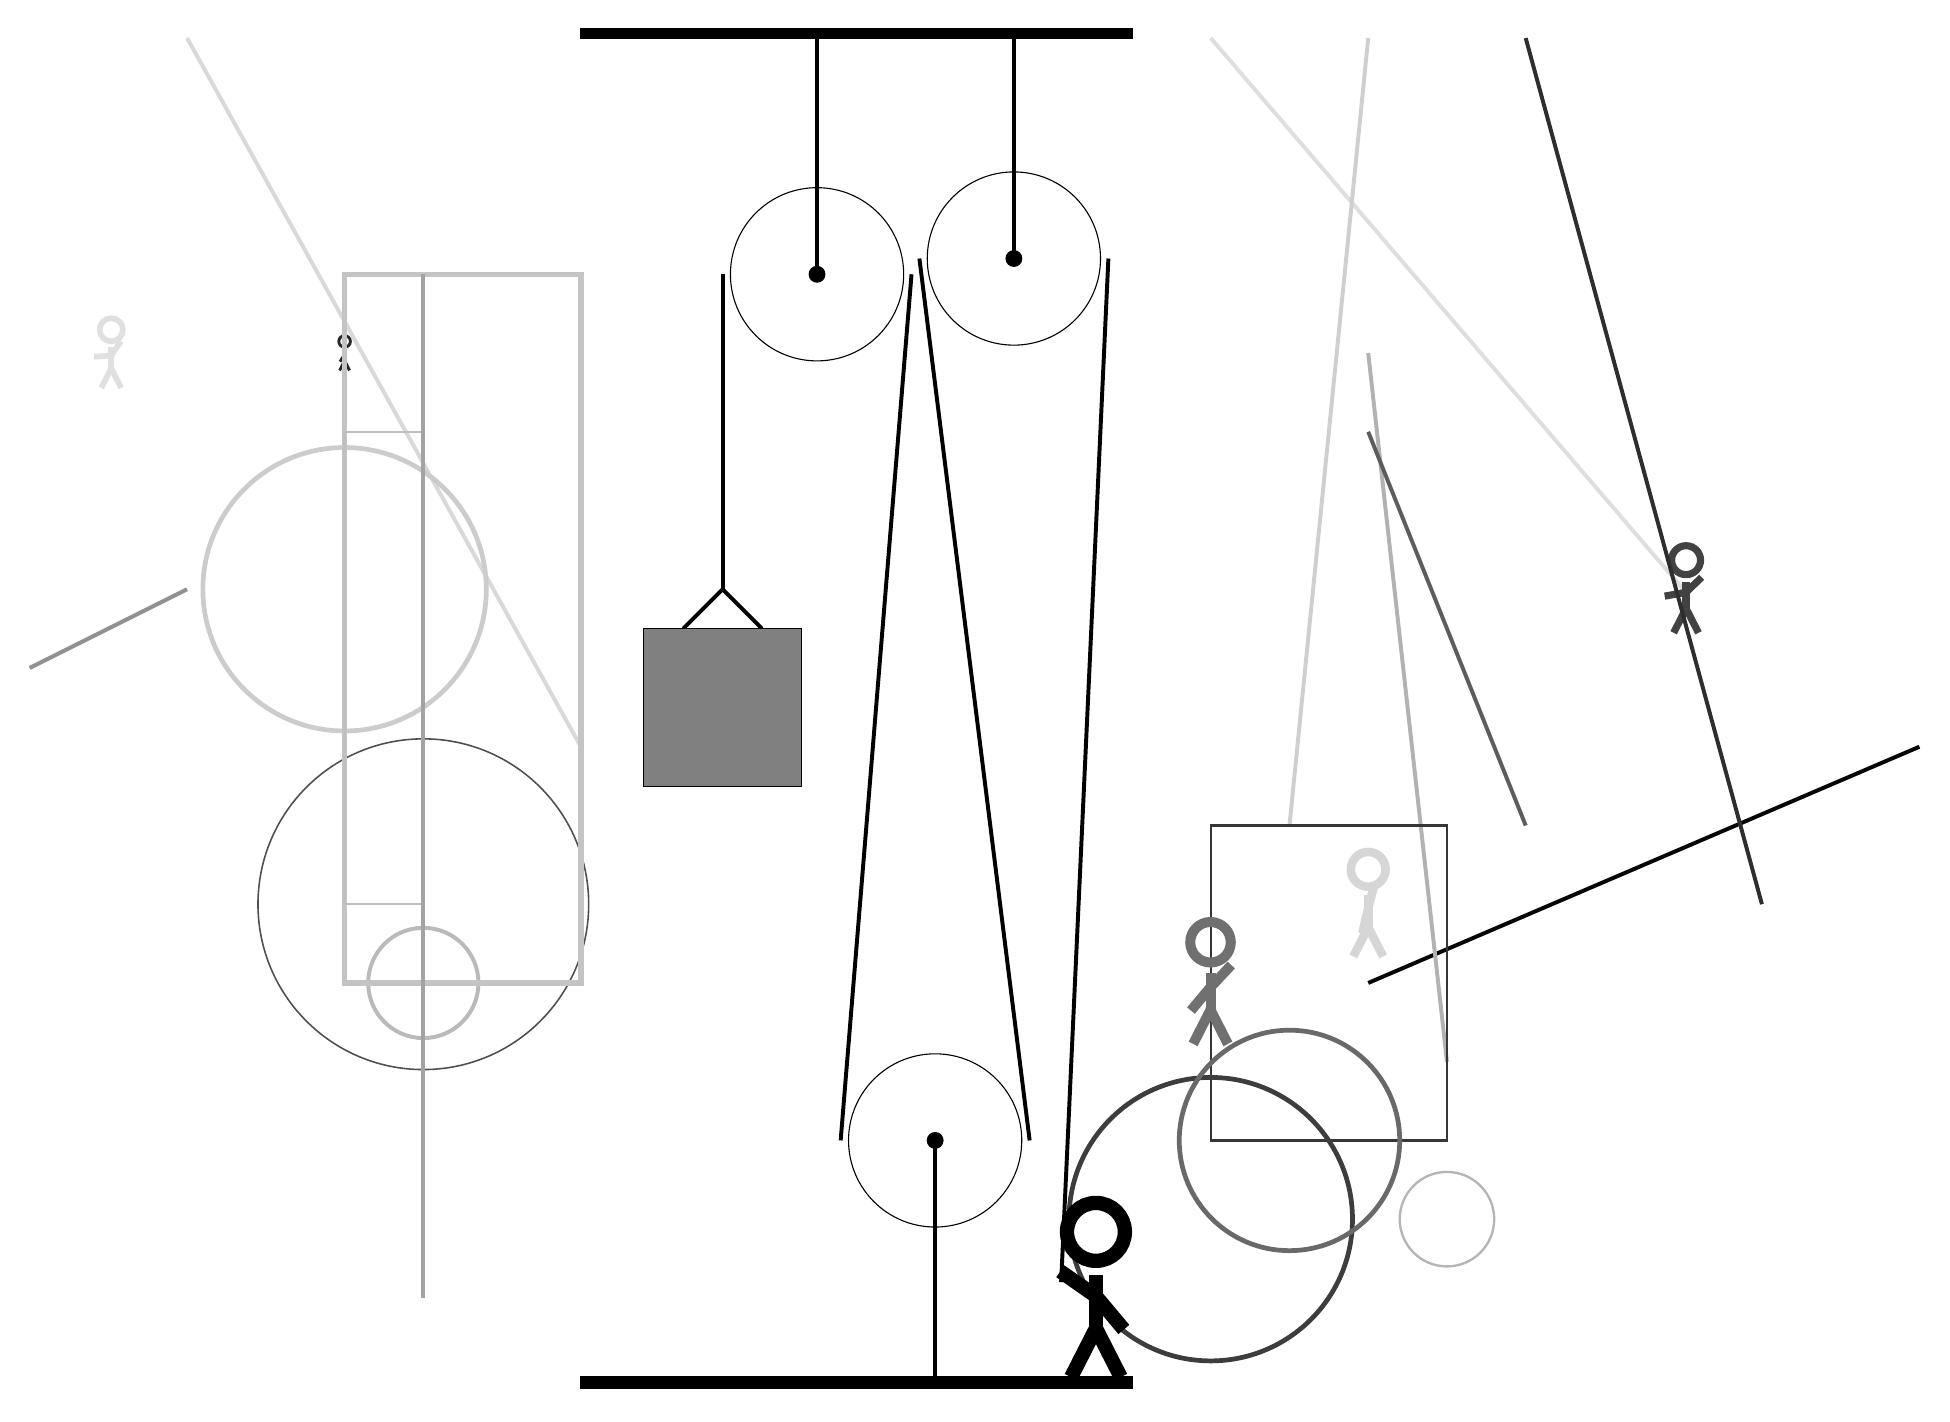
\begin{tikzpicture}
			%%%%% START %%%%%
			
			\draw[fill=black] (-2, 14) rectangle (5, 14.125);
			
			\draw (1, 11) circle (1.1);
			\draw[fill=black] (1, 11) circle (0.1);
			\draw[line width=0.5mm]  (1, 14) -- (1, 11);
			
			\draw [line width=0.2mm, color=black!69](-4, 3) circle (2.1);
			
			\draw [line width=0.5mm, color=black!27](-4, 2) circle (0.7);
			\draw[line width=0.5mm, color=black!13](6, 14) -- (12, 7);
			\draw[line width=0.5mm, color=black!15](-7, 14) -- (-2, 5);
			\node[line width=0.5mm, color=black!12] at (-8, 10) {\Strichmaxerl[4][4][56]};
			\draw [line width=0.6mm, color=black!20](-5, 7) circle (1.8);
			\node[line width=0.6mm, color=black!16] at (8, 3) {\Strichmaxerl[6][77][75]};
			\draw [line width=0.3mm, color=black!29](9, -1) circle (0.6);
			\draw[line width=0.5mm, color=black!98](8, 2) -- (15, 5);
			\draw[line width=0.5mm, color=black!30](8, 10) -- (9, 1);
			\draw[line width=0.5mm, color=black!19](8, 14) -- (7, 4);
			\draw[line width=0.5mm, color=black!64](8, 9) -- (10, 4);
			\draw[line width=0.3mm, color=black!79] (6, 4) rectangle (9, 0);
			\node[line width=0.5mm, color=black!85] at (-5, 10) {\Strichmaxerl[2][58][85]};
			\node[line width=0.2mm, color=black!56] at (6, 2) {\Strichmaxerl[7][50][47]};
			\draw[line width=0.5mm, color=black!43](-7, 7) -- (-9, 6);
			
			\draw [line width=0.6mm, color=black!76](6, -1) circle (1.8);
			\draw[line width=0.7mm, color=black!23] (-2, 2) rectangle (-5, 11);
			\node[line width=0.3mm, color=black!74] at (12, 7) {\Strichmaxerl[5][10][44]};
			\draw [line width=0.6mm, color=black!59](7, 0) circle (1.4);
			\draw[line width=0.5mm, color=black!82](10, 14) -- (13, 3);
			\draw[line width=0.3mm, color=black!25] (-4, 9) rectangle (-5, 3);
			\draw[line width=0.5mm, color=black!36](-4, -2) -- (-4, 11);
			
			\draw[fill=white](2.5, 0) circle (1.1);
			\draw[fill=black] (2.5, 0) circle (0.1);
			\draw[line width=0.5mm]  (2.5, -3) -- (2.5, 0);
			
			\draw[fill=white](3.5, 11.2) circle (1.1);
			\draw[fill=black] (3.5, 11.2) circle (0.1);
			\draw[line width=0.5mm] (3.5, 14) -- (3.5, 11.2);
			
			\draw[line width=0.5mm] (-0.7, 6.5) -- (-0.2, 7.0) -- (0.3, 6.5);
			\draw[fill=black!50] (-1.2, 6.5) rectangle (0.8, 4.5);
			
			\draw[line width=0.5mm] (-0.2, 11) -- (-0.2, 7.0);
			\centerarc[line width=0.5mm](1, 11)(0:180:1.2000000000000002);
			\draw[line width=0.5mm](2.2, 11) -- (1.3, 0);
			\centerarc[line width=0.5mm](2.5, 0)(180:360:1.2000000000000002);
			\draw[line width=0.5mm](3.7, 0) -- (2.3, 11.2);
			\centerarc[line width=0.5mm](3.5, 11.2)(0:180:1.2000000000000002);
			\draw[line width=0.5mm](4.7, 11.2) -- (4.1, -1.8);
			
			\node at (4.5, -1.9) {\Strichmaxerl[10][-35][-50]};
			
			\draw[fill=black] (-2, -3) rectangle (5, -3.15);
			
			%%%%% END %%%%%
		\end{tikzpicture}
	\end{figure}	
\end{document}